\documentclass[10pt]{beamer}

\usepackage[utf8]{inputenc}
\usepackage[spanish, es-tabla]{babel}

\usetheme{metropolis}
\usepackage{appendixnumberbeamer}

\usepackage{booktabs}
\usepackage[scale=2]{ccicons}

\usepackage{pgfplots}
\usepgfplotslibrary{dateplot}

\usepackage{graphicx}

\usepackage{amsmath}
\usepackage{amsfonts}
\usepackage{amssymb}
\usepackage{amsthm}
\usepackage{esvect}

\usepackage{xspace}
\newcommand{\themename}{\textbf{\textsc{metropolis}}\xspace}

\title{The Whale Optimization Algorithm (WOA)}
\author{Ignacio Aguilera Martos}
\date{8 Mayo 2018}
\institute{Metaheurísticas}

\begin{document}

\maketitle

\begin{frame}[fragile]{Contenidos}
  \setbeamertemplate{section in toc}[sections numbered]
  \tableofcontents[hideallsubsections]
\end{frame}

\section{¿Cómo cazan las ballenas jorobadas?}

\begin{frame}[fragile]{Fases de la caza}
	\vspace{10px}
	\pause
	\metroset{block=fill}
	\begin{block}{Fases de la caza}
		\begin{itemize}
			\item Exploración para encontrar presas.
			\pause
			\item Caza de presas.
		\end{itemize}
	\end{block}
	\pause
	\begin{center}
		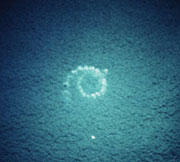
\includegraphics[scale=0.7]{./Imagenes/imagen1.jpg}
		\hspace{10px}
		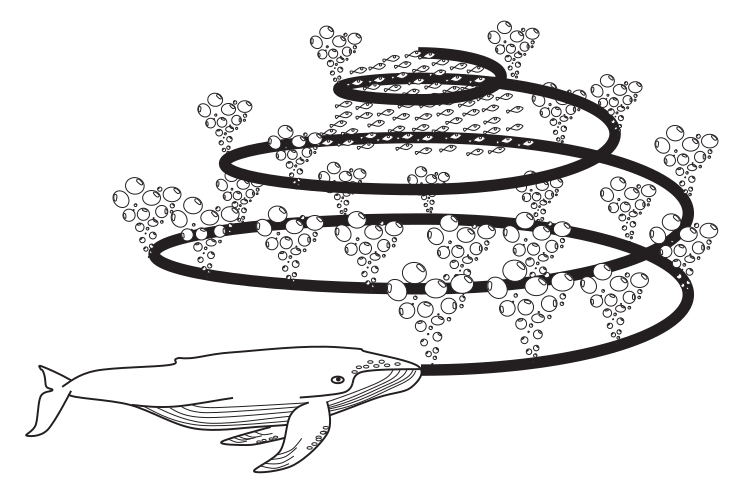
\includegraphics[scale=0.22]{./Imagenes/imagen2.png}
	\end{center}
\end{frame}

\section{Modelo matemático}

\begin{frame}[fragile]{Aproximación a la presa}
	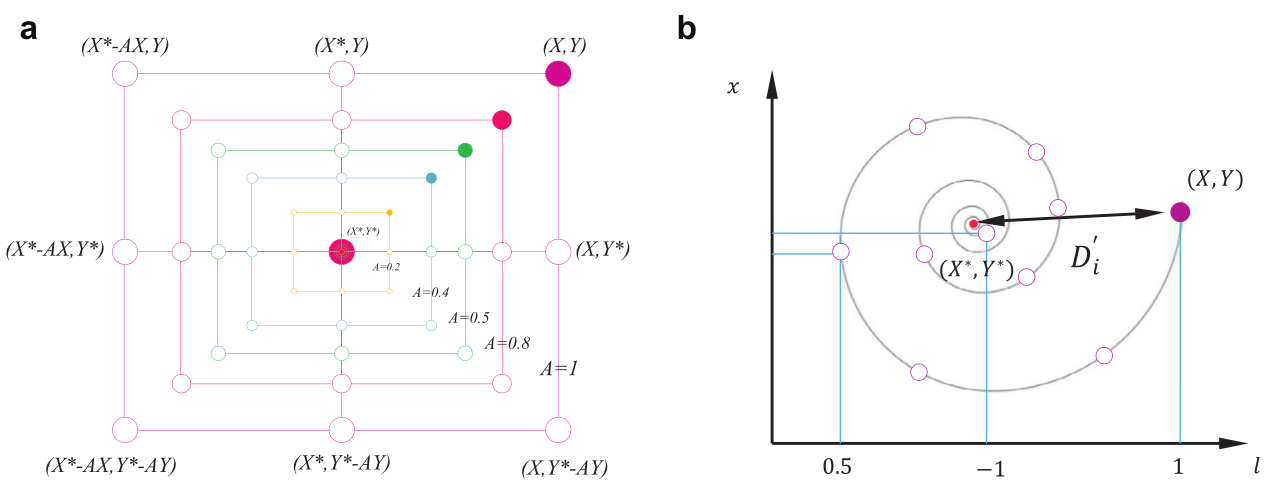
\includegraphics[scale=0.23]{./Imagenes/imagen3.png}
	\pause
	\vspace{5px}
	$D(t) = |\vec{C}\cdot \vec{X^*}(t)-\vec{X}(t)|$ \hspace{20px} $\vec{X}(t+1) = \vec{X^*}(t)-\vec{A}\cdot D(t)$ \\
	\pause
	$D'(t) = |\vec{X^*}(t)-\vec{X}(t)|$ \hspace{20px} $\vec{X}(t+1) = \vec{D'}(t)\cdot e^{bl}\cdot \cos (2\pi l)+\vec{X^*}(t)$ \\
	\vspace{10px}
	$\vec{A} = 2\cdot \vec{a}\cdot \vec{r}-\vec{a}$ \hspace{20px} $\vec{C}=2\cdot \vec{r}$ \\
	\pause
	Donde $X$ es la posición de la ballena, $X^*$ la posición de la presa, $\vec{r}$ un vector aleatorio con valores en el intervalo $[0,1]$ y $a\in [0,2]$ que se decrementa de forma lineal desde 2 hasta 0.
\end{frame}

\begin{frame}[fragile]{Ecuación real del movimiento}
	\pause
	$$
	\vec{X}(t+1)=
	\begin{cases}
		\vec{X}(t+1) = \vec{X^*}(t)-\vec{A}\cdot D(t) & si \ p<0.5\\
		\vec{X}(t+1) = \vec{D'}(t)\cdot e^{bl}\cdot \cos (2\pi l)+\vec{X^*}(t) & si \ p \geq 0.5
	\end{cases}
	$$
	\pause
	Donde p es un número aleatorio en el intervalo $[0,1]$ \\
	\pause
	En caso de no tener presa hacemos el movimiento lineal hacia un vector aleatorio.
\end{frame}

\section{Pseudocódigo}

\begin{frame}[fragile]{Pseudocódigo}
	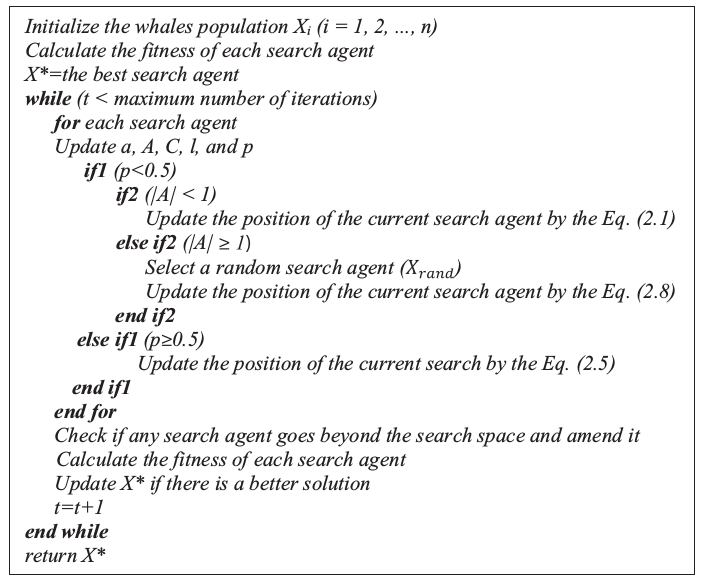
\includegraphics[scale=0.4]{./Imagenes/imagen4.png}
\end{frame}

\begin{frame}[standout]
	\huge Ideas y preguntas.
\end{frame}

\end{document}
